\documentclass[12pt,letterpaper]{article}
\usepackage[utf8]{inputenc}
\usepackage[spanish]{babel}
\usepackage{graphicx}
\usepackage[left=2cm,right=2cm,top=2cm,bottom=2cm]{geometry}
\usepackage{graphicx} % figuras
% \usepackage{subfigure} % subfiguras
\usepackage{float} % para usar [H]
\usepackage{amsmath}
%\usepackage{txfonts}
\usepackage{stackrel} 
\usepackage{multirow}
\usepackage{enumerate} % enumerados
\renewcommand{\labelitemi}{$-$}
\renewcommand{\labelitemii}{$\cdot$}
% \author{}
% \title{Caratula}
\begin{document}

% Fancy Header and Footer
% \usepackage{fancyhdr}
% \pagestyle{fancy}
% \cfoot{}
% \rfoot{\thepage}
%

% \usepackage[hidelinks]{hyperref} % CREA HYPERVINCULOS EN INDICE

% \author{}
\title{Caratula}

\begin{titlepage}
\begin{center}
\large{UNIVERSIDAD PRIVADA-DE-TACNA}\\
\vspace*{-0.025in}
\begin{figure}[htb]
\begin{center}

\includegraphics[width=8cm]{./Imagenes/logo}
\end{center}
\end{figure}
\vspace*{0.15in}
INGENIERIA DE SISTEMAS  \\

\vspace*{0.5in}
\begin{large}
TITULO:\\
\end{large}

\vspace*{0.1in}
\begin{Large}
\textbf{INFORME DE LABORATORIO No 04} \\
\end{Large}

\vspace*{0.3in}
\begin{Large}
\textbf{CURSO:} \\
\end{Large}

\vspace*{0.1in}
\begin{large}
BASE DE DATOS II\\
\end{large}

\vspace*{0.3in}
\begin{Large}
\textbf{DOCENTE(ING):} \\
\end{Large}

\vspace*{0.1in}
\begin{large}
 Patrick Cuadros Quiroga\\
\end{large}

\vspace*{0.2in}
\vspace*{0.1in}
\begin{large}
Integrantes: \\
\begin{flushleft}
Laura Atencio, Nilson Felix		\hfill	(2015053846) \\

\end{flushleft}
\end{large}
\end{center}

\end{titlepage}


\tableofcontents % INDICE
\thispagestyle{empty} % INDICE SIN NUMERO
\newpage
\setcounter{page}{1} % REINICIAR CONTADOR DE PAGINAS DESPUES DEL INDICE

\section{INFORMACIÓN GENERAL} 

\begin{itemize}
\subsection{Objetivos:}
	\item Conocer los fundamentos sobre contenedores y Docker.
	\item Poder instalar correctamente una instancia.
\subsection{Equipos, materiales, programas y recursos utilizados:}
	\item Virtualización activada en el BIOS.
	\item Windows 10 64bit: Pro, Enterprise o Education, con al menos 4GB de RAM.
	\item Docker Desktop
	\item Microsoft SQL Server 2017 o superior

\end{itemize}

\section{MARCO TEORICO} 

\subsection{DOCKER}
Es una plataforma de contener independiente moderna para la innovacion de alta velocidad que permite a las organizaciones crear, compartir y ejecutar sin problemas cualquier aplicación, en cualquier lugar, por ejemplo en la nube hibrida.
Este software de TI, es una tecnología para crear contenedores y/o usar contenedores de Linux.
\\Con DOCKER, puede usar los contenedores como máquinas virtuales extremadamente livianas y modulares. 
 En Docker lo que se hace es usar las funcionalidades del Kernel para encapsular un sistema, de esta forma el proyecto que corre dentro de el no tendrá conocimiento que está en un contenedor. Además, obtiene flexibilidad con estos contenedores: puede crearlos, implementarlos, copiarlos y moverlos de un entorno a otro, lo cual le permite optimizar sus aplicaciones para la nube.
\begin {itemize}
	\item ¿Qué son los contenedores?\\\\
	Docker trabaja con “contenedores de Linux” estos son un conjunto de tecnologías que juntas forman un contenedor en Docker, los conjuntos de tecnologías se llaman:
	\subitem • Namespaces: Permite a la aplicación que corre en un contenedor de Docker tener una vista de los recursos del sistema operativo.
	\subitem • Cgroups: Permite limitar y medir los recursos que se encuentran disponibles en el sistema operativo.
	\subitem • Chroot: Permite tener en el contenedor una vista de un sistema “falso” para el mismo, es decir, crea su propio entorno de ejecución con su propio root y home. \\
	Algunas caracteristicas: 
\subitem • Los contenedores son más livianos ya que trabajan directamente en Kernel que las maquinas virtuales.
\subitem • No es necesario instalar un sistema operativo por contenedor.
\subitem • Menor uso de los recursos de la máquina.
\subitem • Mayor cantidad de contenedores por equipo físico.
\subitem • Mejor portabilidad.\\
	\item Funcionamiento de Docker\\
	\subitem - El propósito de los contenedores es la independencia, es decir, la capacidad de ejecutar varios procesos y aplicaciones por separado para hacer un mejor uso de su infraestructura y, al mismo tiempo, conservar la seguridad que tendría con sistemas separados.\\
	\subitem - Las herramientas del contenedor ofrecen un modelo de implementación basado en imágenes.
	\subitem - Permite compartir una aplicación, o un conjunto de servicios, con todas sus dependencias en varios entornos. \\\\
	\item Ventajas de los contenedores Docker :\\
	\subitem - Modularidad: Se centra en tomar una parte de una aplicación, para actualizarla o repararla, sin necesidad de tomar la aplicación completa.\\
	\subitem - Control de versiones de imágenes y capas: Cada archivo de imagen se compone de una serie de capas y estas van cambiando en una sola imagen. Se crea una capa cuando la imagen cambia y cada vez que se utiliza el comando ejecutar o copiar se crea una nueva capa. 
El control de versiones es inherente a la creación de capas. Cada vez que se produce un cambio nuevo, básicamente, usted tiene un registro de cambios incorporado: control completo de sus imágenes de contenedor.
	\subitem - Restauración: Una imagen tiene capas y cuando no se esta conforme con la actual se puede restaurar a la versión anterior. Esto es compatible con un enfoque de desarrollo ágil y permite hacer realidad la integración e implementación continuas (CI/CD) desde una perspectiva de las herramientas.\\
	\subitem - Implementación rápida: Los contenedores basados en Docker pueden reducir el tiempo de implementación a segundos. debido a que un Sistema Operativo no necesita iniciarse para agregar o mover un contenedor, los tiempos de implementación son sustancialmente inferiores. 
Además se puede crear y destruir la información creada por sus contenedores sin preocupación, de forma fácil y rentable.\\
	
\end{itemize}






\section{PROCEDIMIENTO} 

\begin{itemize}
\subsection{Parte 1: Iniciando Docker:}
	\item Abrir el menu inicio y buscar la aplicación Docker for Windows.
                    \begin{figure}[H]
		\begin{center}
		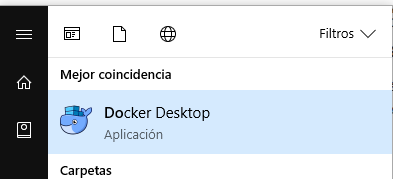
\includegraphics[width=7cm]{./Imagenes/25}
		\end{center}
		\end{figure}
	\item Una vez iniciado se podrá visualizar el icono de Docker en el área de notificación.
   \begin{figure}[H]
		\begin{center}
		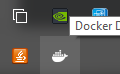
\includegraphics[width=7cm]{./Imagenes/26}
		\end{center}
		\end{figure}
          \item Asimismo se podrá visualizar la ventana de bienvenida.
          \item Ingresar sus credenciales creadas en Docker Hub para iniciar sesión en el aplicativo..
   \begin{figure}[H]
		\begin{center}
		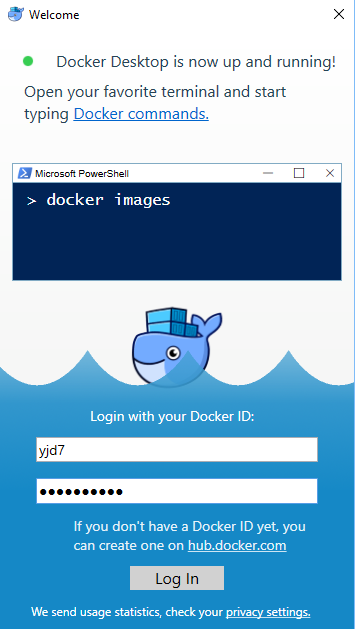
\includegraphics[width=7cm]{./Imagenes/1}
		\end{center}
		\end{figure} 
          \item Ubicar la aplicación PowerShell, ejecutarla como Administrador. En la ventana de comandos de PowerShell escribir lo siguiente: "docker versión"
                       \begin{figure}[H]
		\begin{center}
		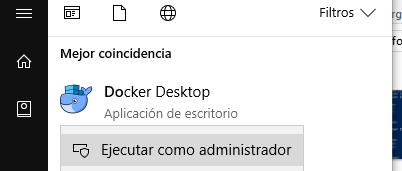
\includegraphics[width=7cm]{./Imagenes/28}
		\end{center}
		\end{figure}   

                      \begin{figure}[H]
		\begin{center}
		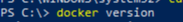
\includegraphics[width=7cm]{./Imagenes/27}
		\end{center}
		\end{figure}   
         \item Verificar que el resultado sea el siguiente.
                     \begin{figure}[H]
		\begin{center}
		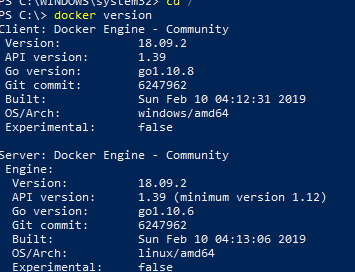
\includegraphics[width=7cm]{./Imagenes/2}
		\end{center}
		\end{figure}   
\subsection{Parte 2: Creando un contenedor con Microsoft SQL Server para Linux}
	\item En la ventana de PowerShell, escribir el siguiente comando:"docker search mssql      
	\item El resultado deberá ser algo similar a lo siguiente.
                     \begin{figure}[H]
		\begin{center}
		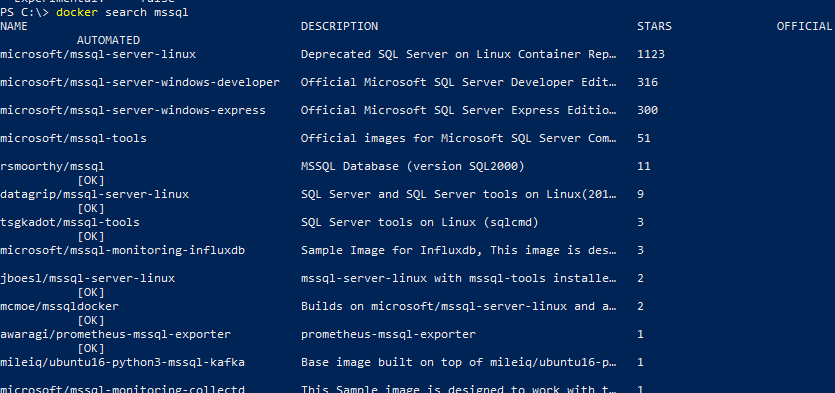
\includegraphics[width=15cm]{./Imagenes/3}
		\end{center}
		\end{figure}   
	\item Ahora ejecutar el comando:"docker pull microsoft/mssql-server-linux"
	\item Lo cual descargará la imagen del contenedor de Microsoft SQL Server en un servidor Linux
                     \begin{figure}[H]
		\begin{center}
		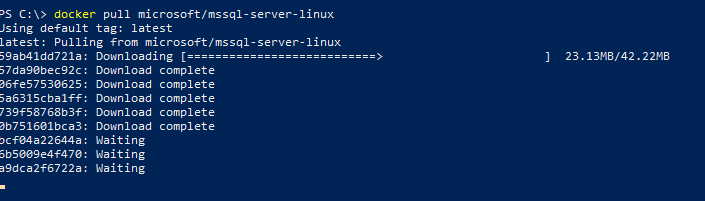
\includegraphics[width=15cm]{./Imagenes/4}
		\end{center}
		\end{figure}   
          \item Proceder a verificar la imagen con el siguiente comando:" docker images"
	\item Lo cual deberá visualizar lo siguiente:
                     \begin{figure}[H]
		\begin{center}
		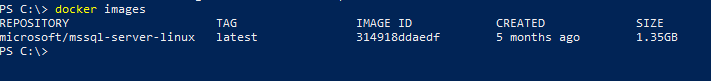
\includegraphics[width=15cm]{./Imagenes/5}
		\end{center}
		\end{figure}   
	\item Seguidamente ejecutar el comando:
                      \begin{figure}[H]
		\begin{center}
		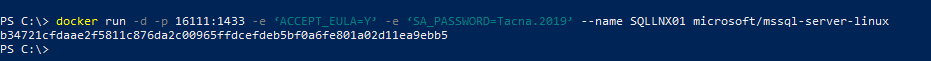
\includegraphics[width=15cm]{./Imagenes/6}
		\end{center}
		\end{figure}   
	\item Como respuesta se visualizará un ID que corresponde al contenedor:
                     \begin{figure}[H]
		\begin{center}
		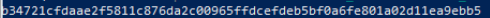
\includegraphics[width=15cm]{./Imagenes/31}
		\end{center}
		\end{figure}   
           \item Verificar que el contenedor se este ejecutando correctamente mediante el comando:" docker ps"       
	\item Si se visualiza un cuadro de dialogo de permisos relacionados al firewall Windows, Aceptarlo para realizar la conexión.El resultado será similar al siguiente:
                     \begin{figure}[H]
		\begin{center}
		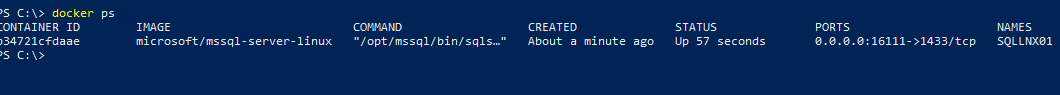
\includegraphics[width=15cm]{./Imagenes/7}
		\end{center}
		\end{figure}   
	\item . Esperar unos segundos e iniciar la aplicación Microsoft SQL Server Management Studio, y conectar con los
siguientes datos:
                      \begin{figure}[H]
		\begin{center}
		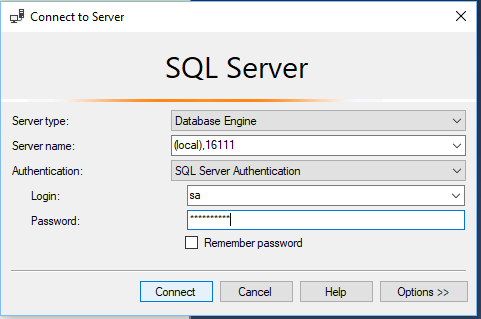
\includegraphics[width=15cm]{./Imagenes/8}
		\end{center}
		\end{figure}   
	\item Iniciar una nueva consulta, escribir y ejecutar lo siguiente:
                     \begin{figure}[H]
		\begin{center}
		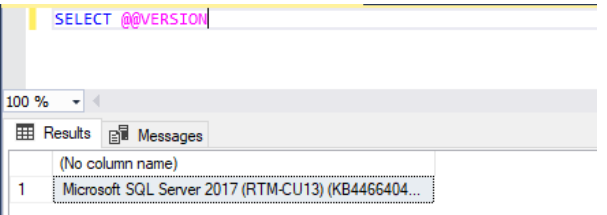
\includegraphics[width=15cm]{./Imagenes/32}
		\end{center}
		\end{figure}   
          \item Deberá retornar algo similar a lo siguiente:
                     \begin{figure}[H]
		\begin{center}
		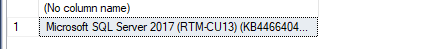
\includegraphics[width=15cm]{./Imagenes/9}
		\end{center}
		\end{figure}   
	\item Cerrar la aplicación Microsoft SQL Server Management Studio.
	\item En PowerShell ejecutar el siguiente comando:" docker rm -f SQLLNX01"
                     \begin{figure}[H]
		\begin{center}
		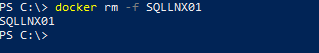
\includegraphics[width=15cm]{./Imagenes/10}
		\end{center}
		\end{figure}   
	\item Verificar la eliminación del contenedor con ejecutando: docker ps
                    \begin{figure}[H]
		\begin{center}
		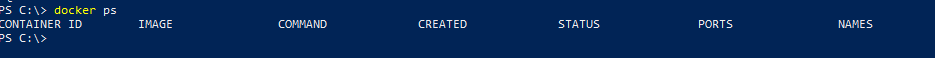
\includegraphics[width=15cm]{./Imagenes/11}
		\end{center}
		\end{figure}   
\subsection{Parte 3: Adicionando persistencia}
	\item En PowerShell ejecutar el siguiente comando.
                     \begin{figure}[H]
		\begin{center}
		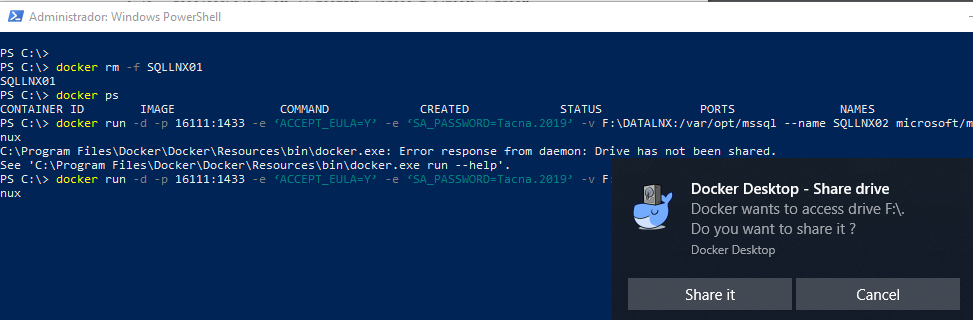
\includegraphics[width=15cm]{./Imagenes/12}
		\end{center}
		\end{figure}   
          \item luego visualizara la siguiente ventana  ingresamos las credenciales.
                     \begin{figure}[H]
		\begin{center}
		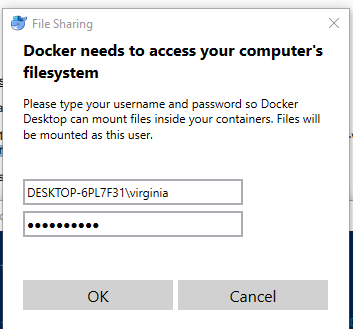
\includegraphics[width=15cm]{./Imagenes/13}
		\end{center}
		\end{figure}   
	\item Como respuesta se visualizará un ID que corresponde al contenedor:
                     \begin{figure}[H]
		\begin{center}
		
\includegraphics[width=15cm]{./Imagenes/14}
		\end{center}
		\end{figure}   
	\item Verificar que el contenedor se este ejecutando correctamente mediante el comando:
                     \begin{figure}[H]
		\begin{center}
		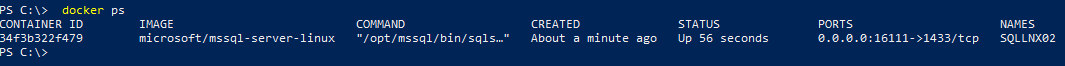
\includegraphics[width=15cm]{./Imagenes/15}
		\end{center}
		\end{figure}   
           \item Esperar unos segundos e iniciar la aplicación Microsoft SQL Server Management Studio, y conectar con los siguientes datos:
                     \begin{figure}[H]
		\begin{center}
		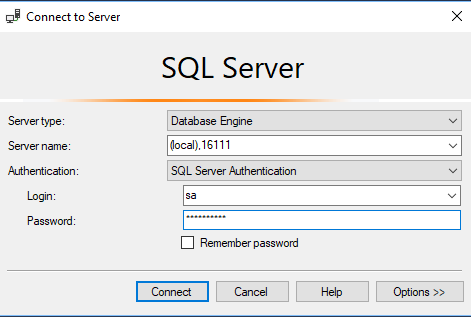
\includegraphics[width=15cm]{./Imagenes/33}
		\end{center}
		\end{figure}   
	\item Generar una base de datos de prueba en la aplicación Microsoft SQL Server Management Studio, según la siguiente imagen mediante el siguiente script:
                     \begin{figure}[H]
		\begin{center}
		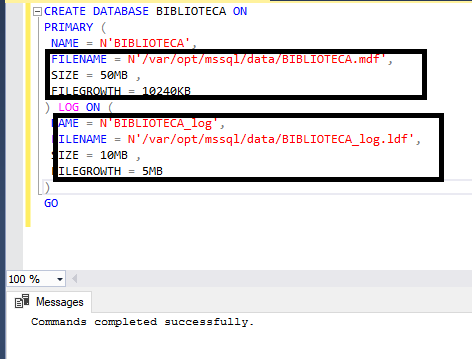
\includegraphics[width=15cm]{./Imagenes/18}
		\end{center}
		\end{figure}   
           \item Verificar el contenido la carpeta DATALNX
                     \begin{figure}[H]
		\begin{center}
		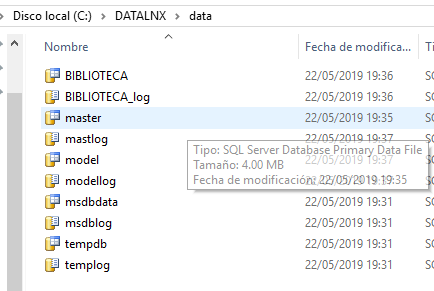
\includegraphics[width=15cm]{./Imagenes/19}
		\end{center}
		\end{figure}   
           \item En PowerShell ejecutar el siguiente comando:"docker rm -f SQLLNX02"
                      \begin{figure}[H]
		\begin{center}
		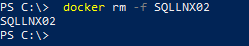
\includegraphics[width=15cm]{./Imagenes/20}
		\end{center}
		\end{figure}   
	\item Verificar la eliminación del contenedor con ejecutando:"docker ps"
                    \begin{figure}[H]
		\begin{center}
		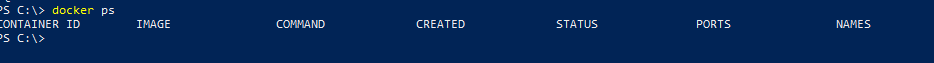
\includegraphics[width=15cm]{./Imagenes/21}
		\end{center}
		\end{figure}   
\item antes se debe compartir o elnazar la carpeta  con Docker
                    \begin{figure}[H]
		\begin{center}
		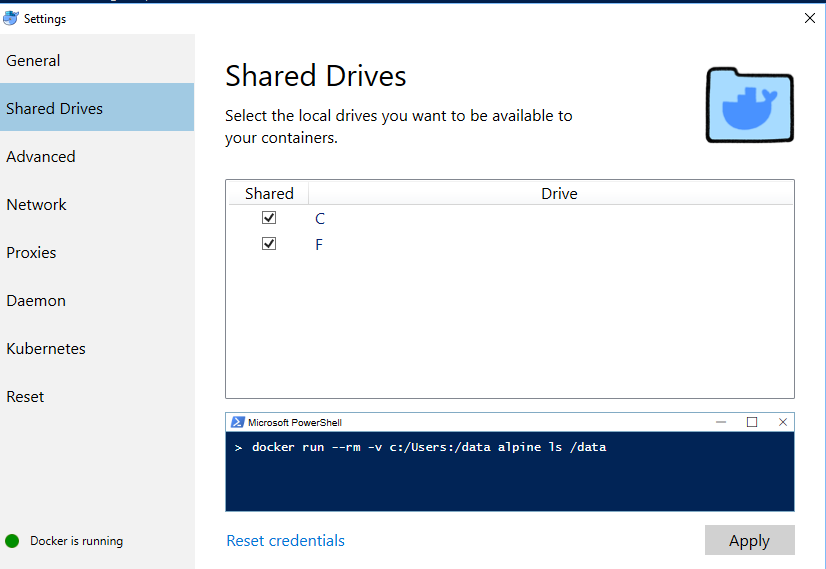
\includegraphics[width=15cm]{./Imagenes/16}
		\end{center}
		\end{figure}   
\subsection{Parte 4: Creando un contenedor con Microsoft SQL Server para Windows}
	\item En el icono de Docker en el área de notificación, hacer click con el botón derecho y utilizar la opción Switch to Windows Containers. Esperar a que Docker se reinicie.
                      \begin{figure}[H]
		\begin{center}
		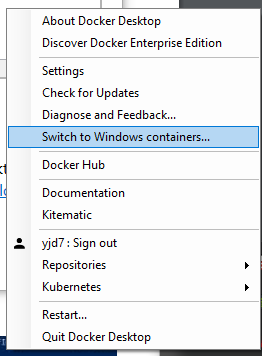
\includegraphics[width=10cm]{./Imagenes/22}
		\end{center}
		\end{figure}   
                      \begin{figure}[H]
		\begin{center}
		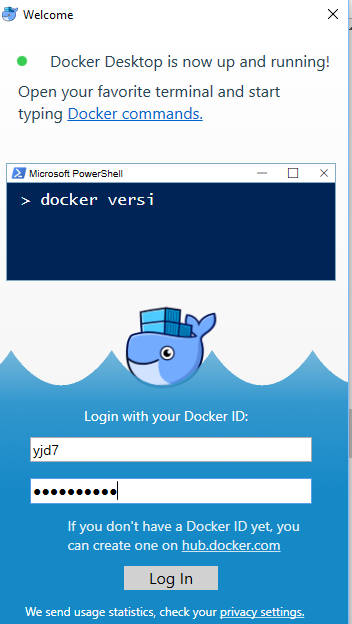
\includegraphics[width=10cm]{./Imagenes/23}
		\end{center}
		\end{figure}   
	\item En la ventana de PowerShell, escribir el siguiente comando:"docker search mssql"           
                       \begin{figure}[H]
		\begin{center}
		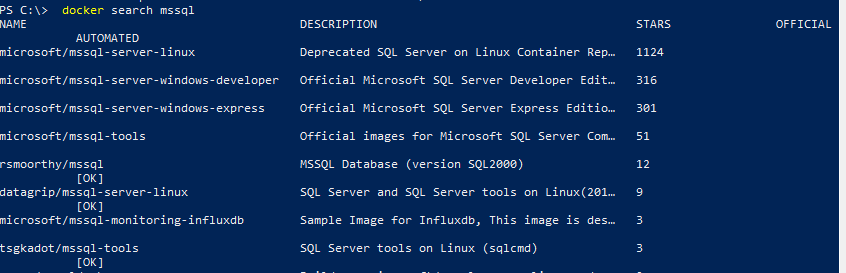
\includegraphics[width=15cm]{./Imagenes/24}
		\end{center}
		\end{figure}   
          \item Ejecutar el siguiente comando; lo cual descargará la imagen del contenedor de Microsoft SQL Server en un servidor Linux.
		\begin{figure}[H]
		\begin{center}
		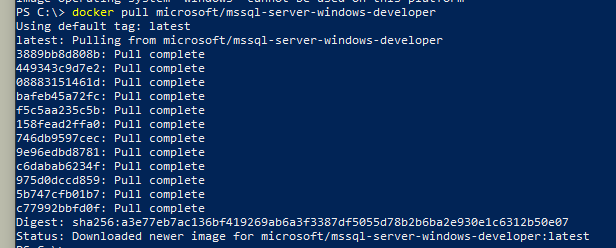
\includegraphics[width=15cm]{./Imagenes/c1}
		\end{center}
		\end{figure}  
         \item Proceder a verificar la imagen con el siguiente comando:
		\begin{figure}[H]
		\begin{center}
		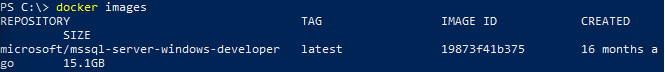
\includegraphics[width=15cm]{./Imagenes/c2}
		\end{center}
		\end{figure}  
          \item Seguidamente ejecutar el comando; como respuesta se visualizará un ID que corresponde al contenedor
		\begin{figure}[H]
		\begin{center}
		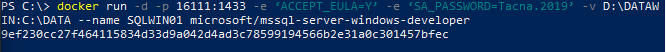
\includegraphics[width=15cm]{./Imagenes/c3}
		\end{center}
		\end{figure}  
          \item Repetir el paso 10 y verificar que el contenedor este ejecutándose
		\begin{figure}[H]
		\begin{center}
		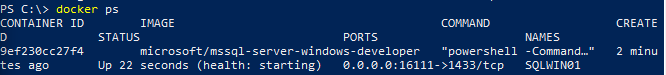
\includegraphics[width=15cm]{./Imagenes/c4}
		\end{center}
		\end{figure}  
          \item Repetir el paso 11 y conectar al servidor
		\begin{figure}[H]
		\begin{center}
		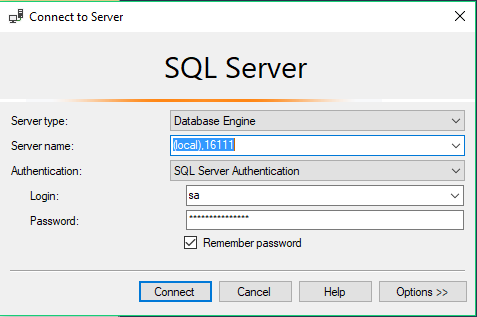
\includegraphics[width=15cm]{./Imagenes/c5}
		\end{center}
		\end{figure}  
         \item Iniciar una nueva consulta, escribir y ejecutar lo siguiente:
		\begin{figure}[H]
		\begin{center}
		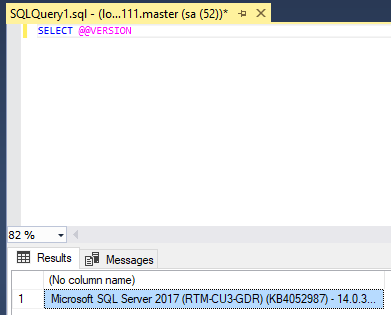
\includegraphics[width=10cm]{./Imagenes/c6}
		\end{center}
		\end{figure}  
          \item Generar una base de datos de prueba en la aplicación Microsoft SQL Server Management Studio
		\begin{figure}[H]
		\begin{center}
		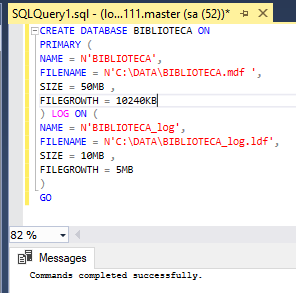
\includegraphics[width=10cm]{./Imagenes/c7}
		\end{center}
		\end{figure}  
          \item Verificar el contenido de la carpeta DATAWIN
		\begin{figure}[H]
		\begin{center}
		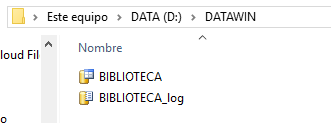
\includegraphics[width=12cm]{./Imagenes/c8}
		\end{center}
		\end{figure}  
         \item En PowerShell ejecutar el siguiente comando y verificar la eliminación del contenedor con ejecutando
		\begin{figure}[H]
		\begin{center}
		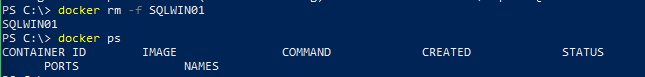
\includegraphics[width=15cm]{./Imagenes/c9}
		\end{center}
		\end{figure}  
          \item Cerrar la aplicación Microsoft SQL Server Management Studio.
       
\end{itemize}
		
\section{ANALISIS E INTERPRETACION DE RESULTADOS} 


\subsection{Parte 1: Actividades Encargadas}
	\begin{itemize}
		\item ¿Con qué comando(s) exportaría la imagen de Docker de Microsoft SQL Server a otra PC o servidor?
                      \begin{figure}[H]
		\begin{center}
		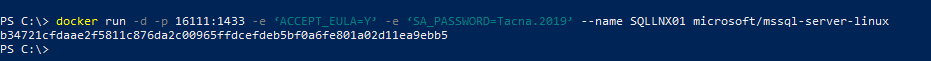
\includegraphics[width=15cm]{./Imagenes/6}
		\end{center}
		\end{figure} 
		\item ¿Con qué comando(s) podría generar dos volúmenes para un contenedor para distribuir en un volumen el Archivo de Datos (.mdf) y en otro el Archivo Log (.ldf)? 
                     \begin{figure}[H]
		\begin{center}
		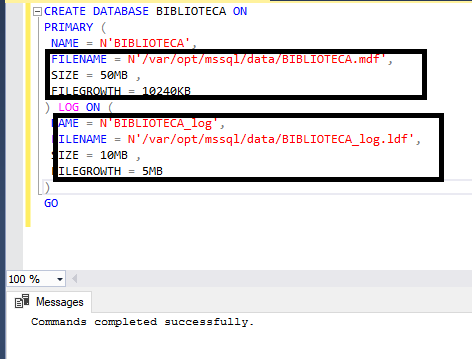
\includegraphics[width=7cm]{./Imagenes/18}
		\end{center}
		\end{figure} 
		\item Genere un nuevo contenedor y cree la base de datos con las siguientes características.
                      \begin{figure}[H]
		\begin{center}
		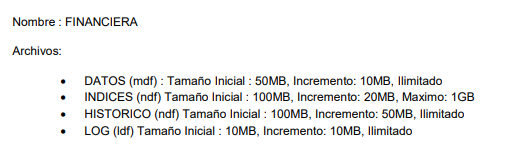
\includegraphics[width=7cm]{./Imagenes/30}
		\end{center}
		\end{figure} 
		\item  ¿Cuál sería el script SQL que generaría esta base de datos?
\begin{figure}[H]
		\begin{center}
		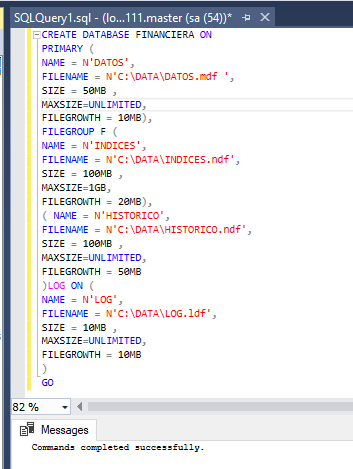
\includegraphics[width=10cm]{./Imagenes/t4}
		\end{center}
		\end{figure}
	\end{itemize}




\section{CONCLUSIONES}
\begin{itemize}
	\item En conclusión hemos observado y experimentado con docker, y nos resulta que es muy util al momento de instalar multiples bases de datos y que no existe la necesidad de armar o instalar múltipler ordenadores físicos o virtuales.
	
	\item Es por eso que resulta factible en muchos aspectos como migrar de version, tener varias bases de datos disponibles o además que existieran y comparen diferentes versiones de bases de datos a la vez
\end{itemize}

\newpage

\section{REFERENCIAS} 

\begin{itemize}
	\item [[ 1]] Hat, R. (2017). ¿Qué es Docker?. Recuperado de https://www.redhat.com/es/topics/containers/what-is-docker
	\item  [[ 2]] Why Docker? | Docker. (2017). Recuperado de https://www.docker.com/why-docker
 	\item   [[ 3]] Araujo, J. (2017). ¿Qué es Docker? ¿Que son los contenedores? y ¿Por que no usar VMs?. Recuperado de https://platzi.com/contributions/guia-del-curso-de-docker/
	\item  [[ 4]]  Oterino, A. (2015). ¿Qué es Docker? ¿Para qué se utiliza? Explicado de forma sencilla. Recuperado de https://www.javiergarzas.com/2015/07/que-es-docker-sencillo.html
\end{itemize}




\end{document}
